% Editable native annotations around unchanged verified IDE photographs.
\par
\begin{figure}[htbp]
\centering
\sbox0{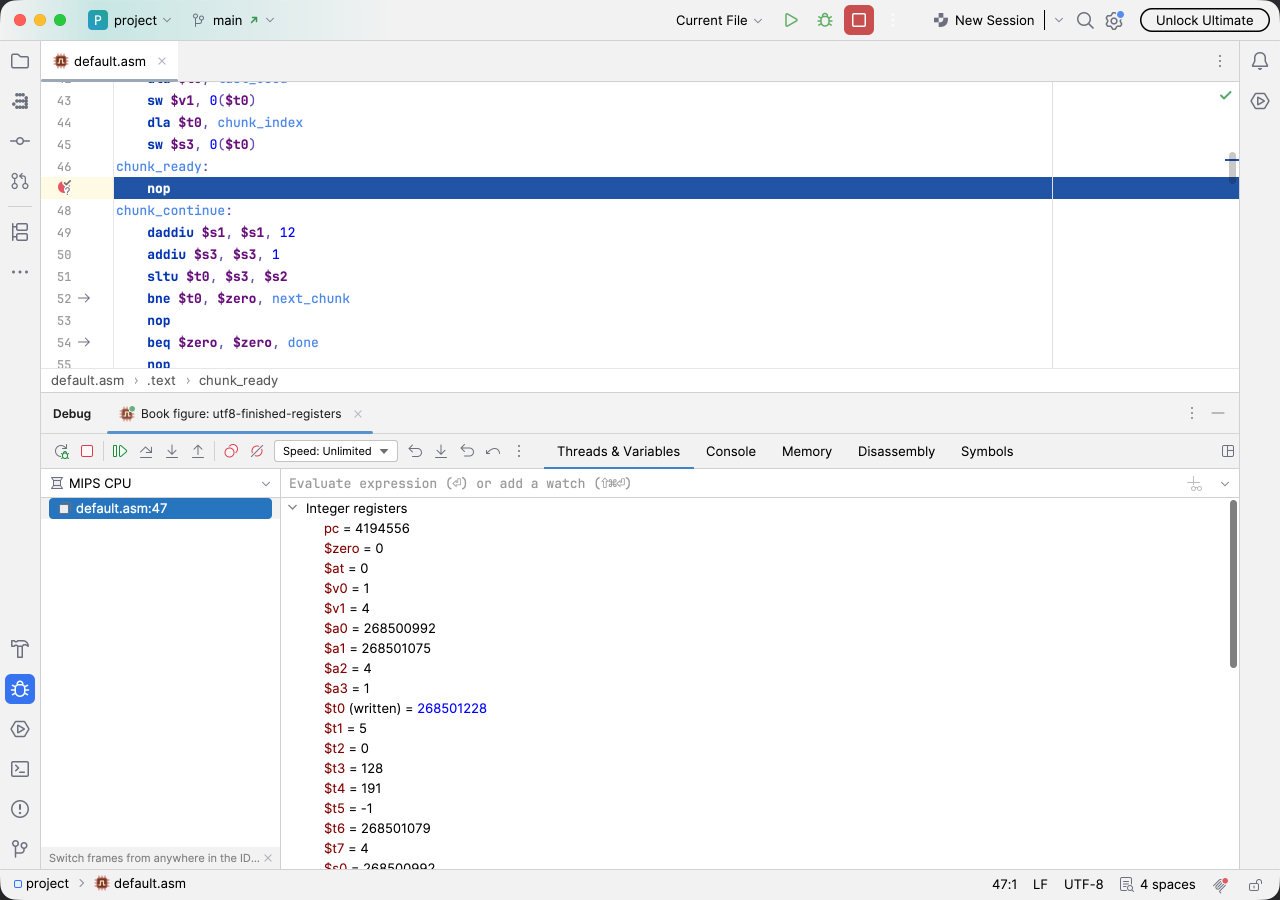
\includegraphics[artifact]{packages/015-utf8-scanner/captures/f02-finished/registers.png}}
\sbox2{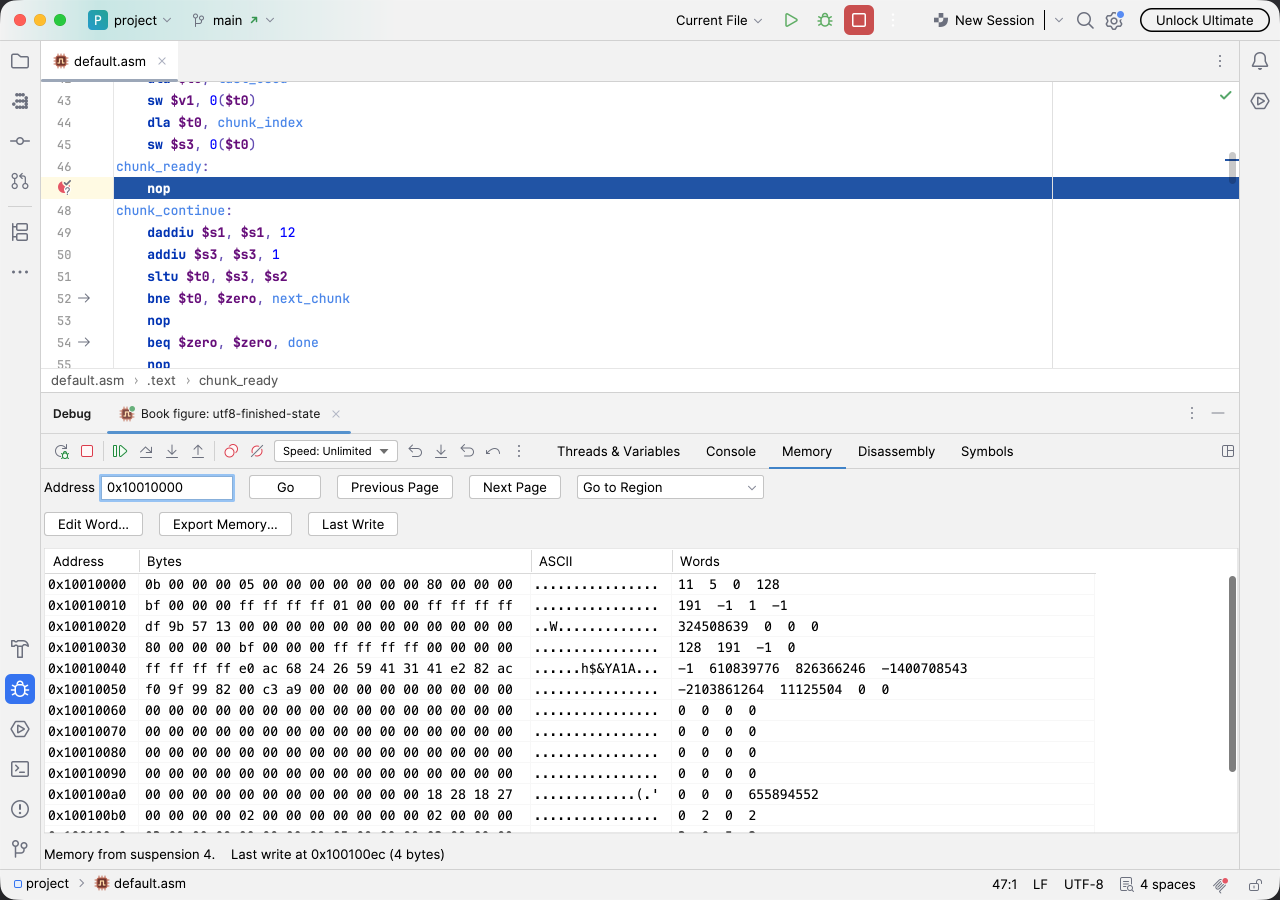
\includegraphics[artifact]{packages/015-utf8-scanner/captures/f02-finished/state.png}}
\sbox4{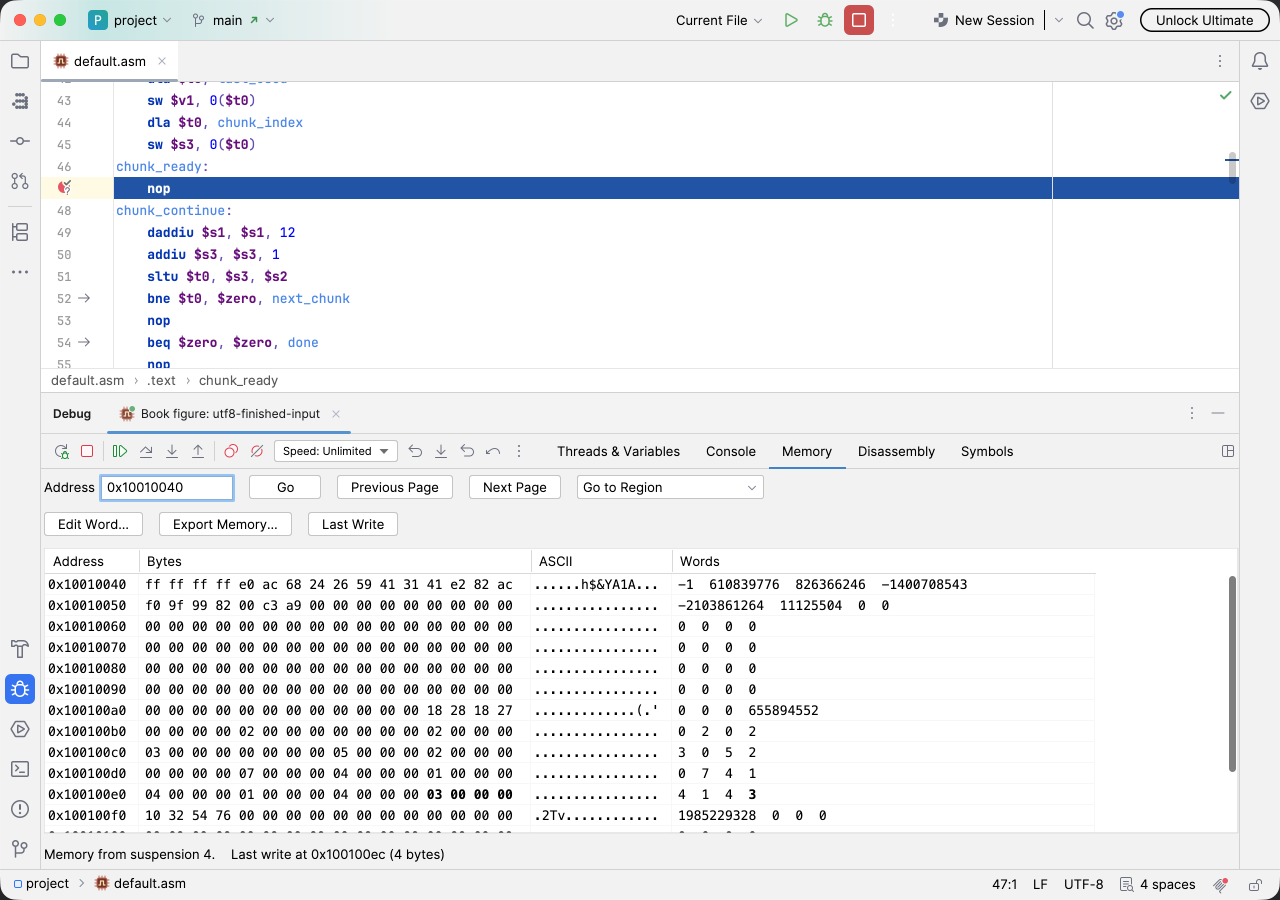
\includegraphics[artifact]{packages/015-utf8-scanner/captures/f02-finished/input.png}}
\edef\MARSutffinishedsourceLeft{\the\dimexpr0.036718750\wd0\relax}
\edef\MARSutffinishedsourceBottom{\the\dimexpr0.774444444\ht0\relax}
\edef\MARSutffinishedsourceRight{\the\dimexpr0.713281250\wd0\relax}
\edef\MARSutffinishedsourceTop{\the\dimexpr0.147777778\ht0\relax}
\edef\MARSutffinishedregistersLeft{\the\dimexpr0.246093750\wd0\relax}
\edef\MARSutffinishedregistersBottom{\the\dimexpr0.312222222\ht0\relax}
\edef\MARSutffinishedregistersRight{\the\dimexpr0.553906250\wd0\relax}
\edef\MARSutffinishedregistersTop{\the\dimexpr0.640000000\ht0\relax}
\edef\MARSutffinishedstateLeft{\the\dimexpr0.034375000\wd2\relax}
\edef\MARSutffinishedstateBottom{\the\dimexpr0.311111111\ht2\relax}
\edef\MARSutffinishedstateRight{\the\dimexpr0.584375000\wd2\relax}
\edef\MARSutffinishedstateTop{\the\dimexpr0.608888889\ht2\relax}
\edef\MARSutffinishedinputLeft{\the\dimexpr0.034375000\wd4\relax}
\edef\MARSutffinishedinputBottom{\the\dimexpr0.311111111\ht4\relax}
\edef\MARSutffinishedinputRight{\the\dimexpr0.584375000\wd4\relax}
\edef\MARSutffinishedinputTop{\the\dimexpr0.608888889\ht4\relax}
\begin{tikzpicture}[alt={Four annotated details after chunk index three. Return status one and used four accompany state total eleven, scalar count five, need zero, ordinary bounds 128 and 191, start minus one, finished status one and error minus one. The input contains A, U+20AC, U+1F642, U+0000 and U+00E9.}]
\node[anchor=north west,inner sep=0,font=\small\bfseries] (source-title) at (6mm,0) {Next instruction after publication};
\node[anchor=north west,inner sep=0] (source) at ([yshift=-1mm]source-title.south west) {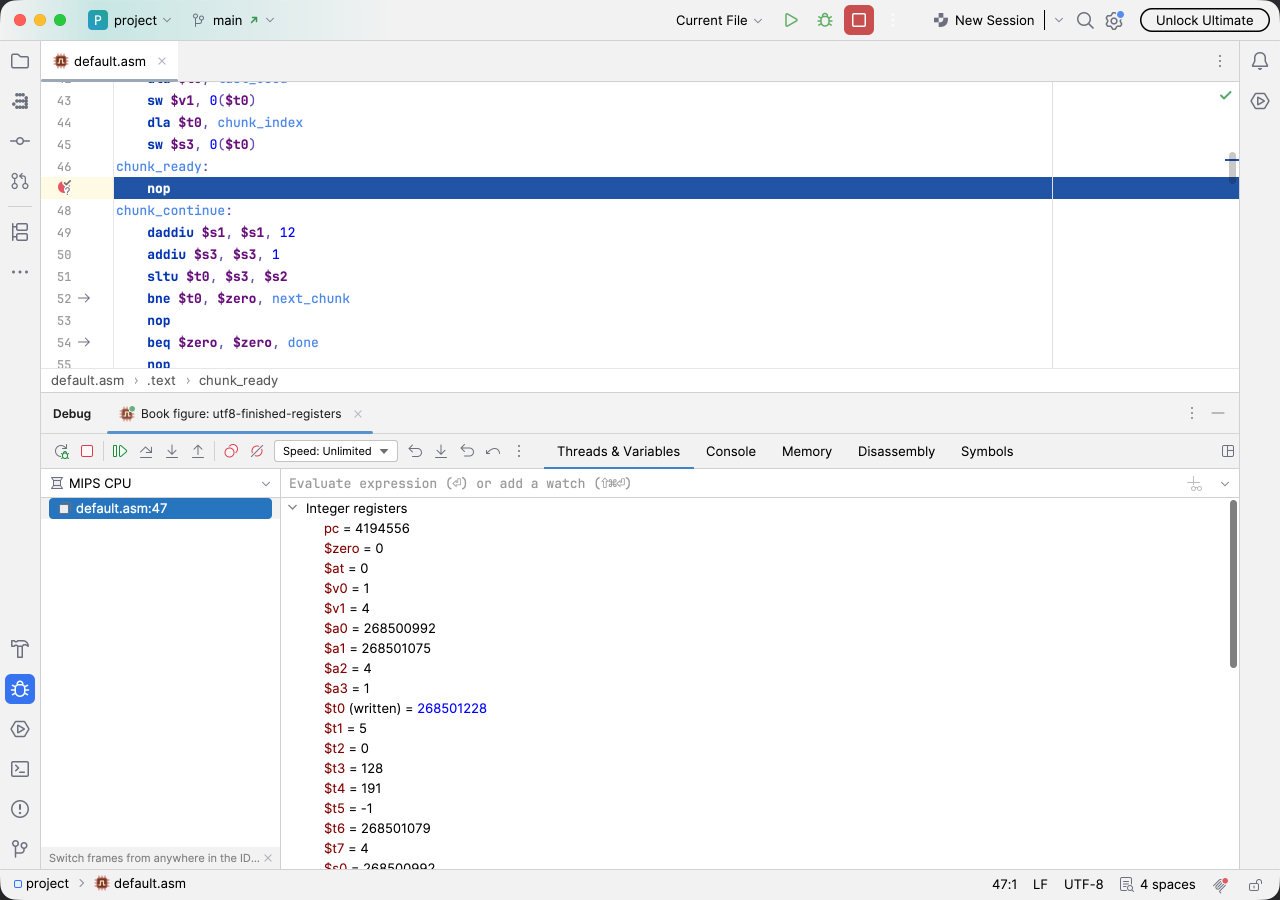
\includegraphics[width=0.54\linewidth,artifact,trim={\MARSutffinishedsourceLeft{} \MARSutffinishedsourceBottom{} \MARSutffinishedsourceRight{} \MARSutffinishedsourceTop{}},clip]{packages/015-utf8-scanner/captures/f02-finished/registers.png}};
\begin{scope}[shift={(source.south west)},x={($(source.south east)-(source.south west)$)},y={($(source.north west)-(source.south west)$)}]
\draw[black,line width=0.7pt] (0.215625000,0.057142857) rectangle (0.384375000,0.371428571);
\node[draw=black,fill=white,circle,inner sep=1.5pt,font=\footnotesize] at ($(0.215625000,0.371428571)+(-3mm,0)$) {1};
\end{scope}
\node[anchor=north west,inner sep=0,font=\small\bfseries] (registers-title) at (0.58\linewidth,0 |- source-title.north) {Signed return values};
\node[anchor=north west,inner sep=0] (registers) at ([yshift=-1mm]registers-title.south west) {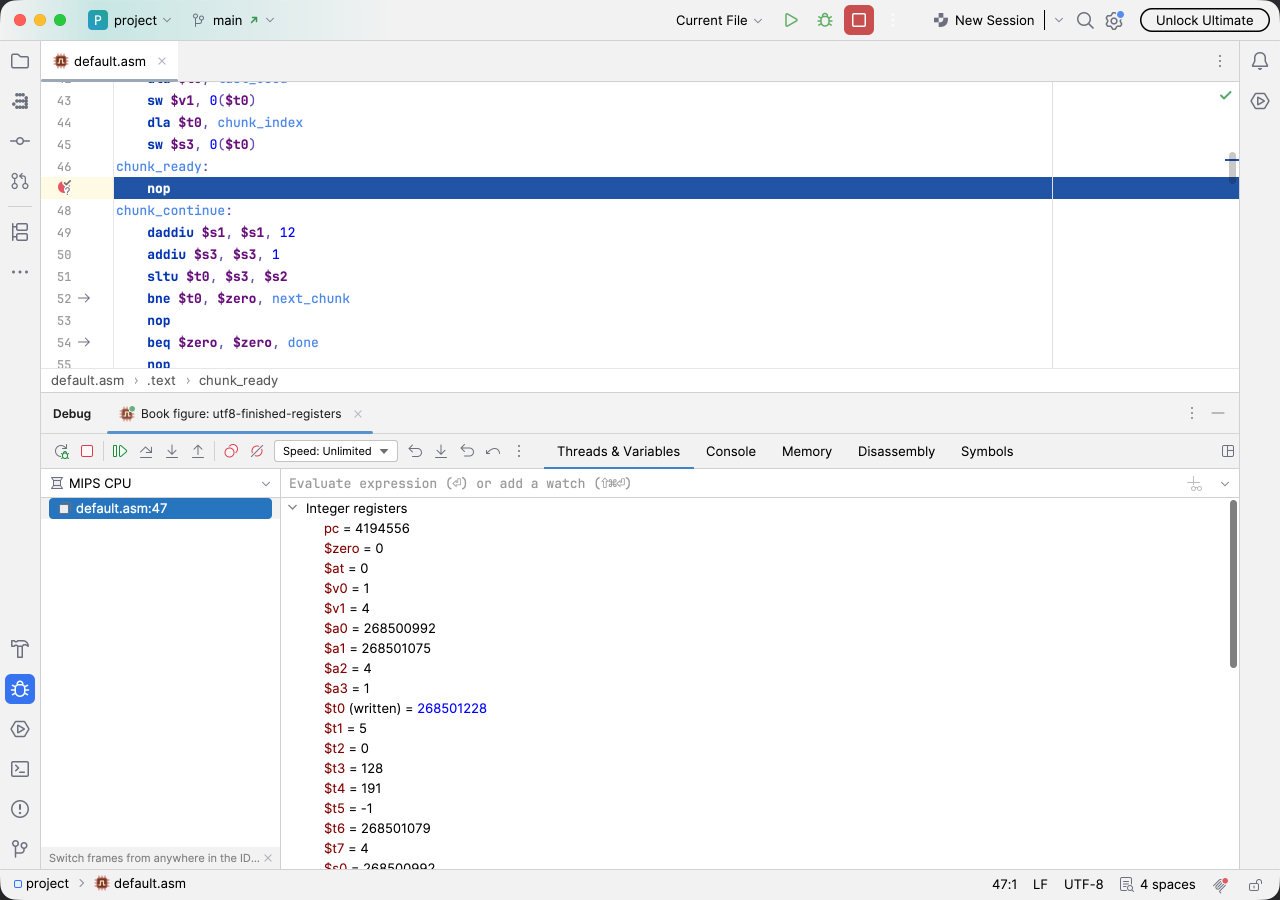
\includegraphics[width=0.42\linewidth,artifact,trim={\MARSutffinishedregistersLeft{} \MARSutffinishedregistersBottom{} \MARSutffinishedregistersRight{} \MARSutffinishedregistersTop{}},clip]{packages/015-utf8-scanner/captures/f02-finished/registers.png}};
\begin{scope}[shift={(registers.south west)},x={($(registers.south east)-(registers.south west)$)},y={($(registers.north west)-(registers.south west)$)}]
\draw[black,line width=0.7pt] (0.023437500,0.023255814) rectangle (0.218750000,0.953488372);
\node[draw=black,fill=white,circle,inner sep=1.5pt,font=\footnotesize] at ($(0.023437500,0.953488372)+(-3mm,0)$) {2};
\end{scope}
\node[anchor=north west,inner sep=0,font=\small\bfseries] (state-title) at ([yshift=-3mm]source.south west) {Stream state: eight little-endian words};
\node[anchor=north west,inner sep=0] (state) at ([yshift=-1mm]state-title.south west) {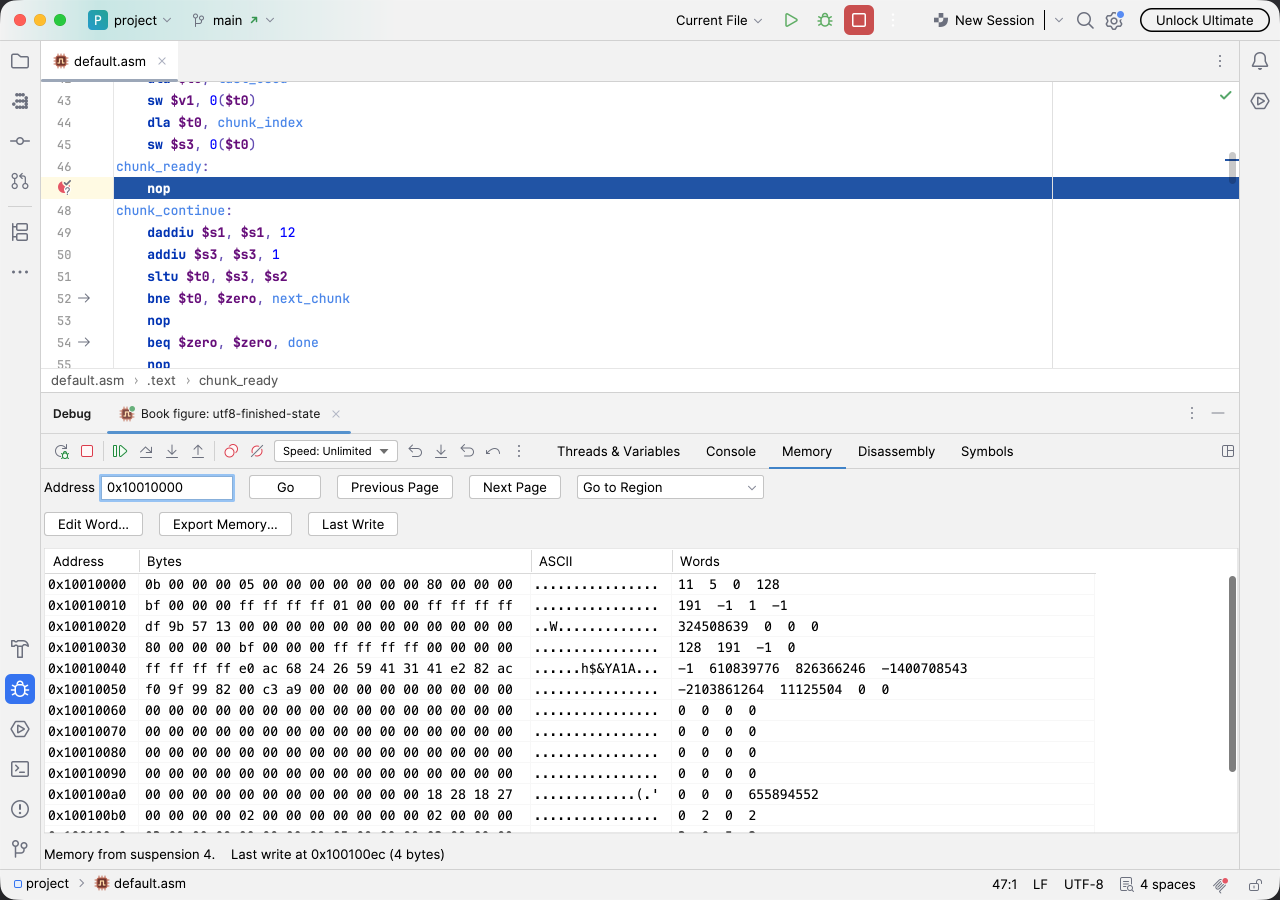
\includegraphics[width=0.84\linewidth,artifact,trim={\MARSutffinishedstateLeft{} \MARSutffinishedstateBottom{} \MARSutffinishedstateRight{} \MARSutffinishedstateTop{}},clip]{packages/015-utf8-scanner/captures/f02-finished/state.png}};
\begin{scope}[shift={(state.south west)},x={($(state.south east)-(state.south west)$)},y={($(state.north west)-(state.south west)$)}]
\draw[black,line width=0.7pt] (0.194672131,0.055555556) rectangle (0.997950820,0.638888889);
\node[draw=black,fill=white,circle,inner sep=1.5pt,font=\footnotesize] at ($(0,0.638888889)+(-3mm,0)$) {3};
\end{scope}
\node[anchor=north west,inner sep=0,font=\small\bfseries] (input-title) at ([yshift=-3mm]state.south west) {Mapped input and neighboring words};
\node[anchor=north west,inner sep=0] (input) at ([yshift=-1mm]input-title.south west) {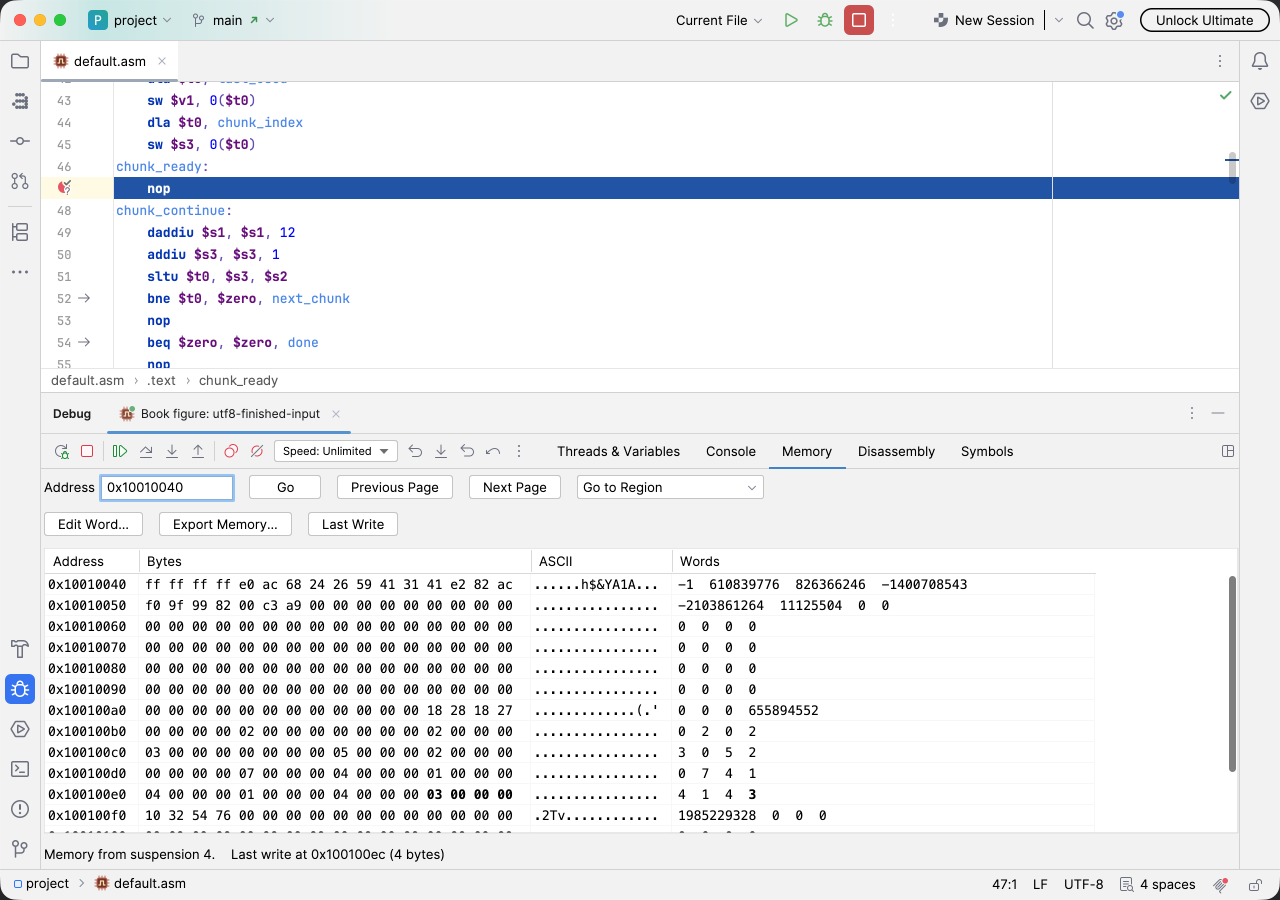
\includegraphics[width=0.84\linewidth,artifact,trim={\MARSutffinishedinputLeft{} \MARSutffinishedinputBottom{} \MARSutffinishedinputRight{} \MARSutffinishedinputTop{}},clip]{packages/015-utf8-scanner/captures/f02-finished/input.png}};
\begin{scope}[shift={(input.south west)},x={($(input.south east)-(input.south west)$)},y={($(input.north west)-(input.south west)$)}]
\draw[black,line width=0.7pt] (0.194672131,0.055555556) rectangle (0.997950820,0.638888889);
\node[draw=black,fill=white,circle,inner sep=1.5pt,font=\footnotesize] at ($(0,0.638888889)+(-3mm,0)$) {4};
\end{scope}
\end{tikzpicture}
\par\smallskip
\begin{minipage}{\linewidth}
\small
\begin{enumerate}
\setlength{\itemsep}{2pt}
\setlength{\parsep}{0pt}
\item This stop follows chunk index 3, the fourth call. Its final flag declares that no further stream bytes will arrive. Completion is decided after processing that chunk; the visible \texttt{nop} is the next instruction after the call and result publication.
\item \texttt{\$v0 = 1} reports a finished stream. \texttt{\$v1 = 4} counts the four bytes accepted by this call: \texttt{82 00 c3 a9}. The first of those bytes completes a sequence retained from earlier calls. A byte accepted now can finish a scalar whose lead arrived earlier.
\item The state words are $[11,5,0,128,191,-1,1,-1]$. All eleven bytes were accepted and five scalar values completed. Need zero and start $-1$ identify no pending sequence; status 1 records final completion and error $-1$ records no error. The ordinary bounds remain stored, but this terminal state accepts no further calls.
\item From \texttt{0x1001004c}, the eleven input bytes encode U+0041, U+20AC, U+1F642, U+0000 and U+00E9. Byte \texttt{00} at stream offset 8 is U+0000 and contributes one scalar; it is not a terminator for this length-delimited interface. The following \texttt{c3 a9} is still processed. Scalar count is distinct from byte count and from a count of displayed glyphs.
\end{enumerate}
\end{minipage}
\caption{The final chunk completes an eleven-byte stream containing five scalar values.}
\label{capture:015-utf8-scanner-f02-finished}
\label{utf8-f02-finished}
\end{figure}
\par
